% ch-parallel.tex -- shared-memory parallelism, what scales and what does not
\chapter{並列実行}
\label{ch:parallel}

YuzenはOpenMPで並列化している。本章では、並列化で得られるものと得られないもの、
指定すべきスレッド数を述べる。正直なところ、答えはケースによって異なるので、実測の結果も
示す。

\begin{warn}[分散メモリ並列は存在しない]
  \textbf{Yuzenは共有メモリ並列のみである。MPIはサポートしておらず、MPI版の予定も
  ない。}一回の計算は一台の計算機上の一つのプロセスであり、その中で複数のスレッドを
  使う。したがって、解ける問題の大きさは単一ノードのメモリで決まり、ノードを足しても
  大きくはできない。また、クラスターは\emph{複数のケースを同時に}（ケースごとに一つの
  プロセスで）実行する用途にしか役立たない。もっとも、もともとそのほうが効率のよい
  使い方である。一つのケースを並列化しても、独立したケースを並べて流す場合ほどには
  スケールしないからである。
\end{warn}

\section{スレッド数の選び方}
\label{sec:parallel:threads}

スレッド数は、通常どおり\env{OMP\_NUM\_THREADS}で指定する。入力ファイルには
対応するキーはない。

\begin{shell}
OMP_NUM_THREADS=2 ./build/bin/yuzen cases/leveling_2d_fine_reg.toml
\end{shell}

\begin{warn}[物理コア数を超えるスレッドを指定してはならない]
  オーバーサブスクリプションによる損失は小さくない。致命的である。
  \SI{2.1}{\giga\hertz}の2コアのXeonで\file{leveling\_1d\_reg}を四スレッドで実行
  すると、一スレッドの三倍から六倍の時間がかかる。開発中に試した自前のバックエンドでは、
  同じ理由で十倍遅くなった（一スレッドの\SI{9.4}{\second}に対して\SI{93}{\second}）。
  \env{OMP\_NUM\_THREADS}は物理コア数以下に設定し、既定値に頼ってはならない。ハイパー
  スレッドを報告する計算機では、既定値が大きすぎる。
\end{warn}

\begin{warn}[使用中のコアはないものとみなす]
  コアがあっても、ほかの処理（別の計算、ビルド、\code{ctest -j}）が使っていれば、
  同じように極端に遅くなる。OpenMPランタイムは並列ループの終わりごとにスピン待ちを
  行い、1ステップには短い並列ループが何千もある。スレッドがコアの空きを待つと、
  ループのたびにスケジューラーのタイムスライス一つ分を失う。2コアの計算機でコアが一つ
  使用中のとき、\code{concz\_vs\_wm}は二スレッドで\SI{246}{\second}かかった。
  \env{OMP\_WAIT\_POLICY=passive}とすると\SI{5}{\second}であった。計算機を共有する場合は、
  スレッド数を空いているコアの数までにとどめるか、
  \env{OMP\_WAIT\_POLICY=passive}を設定する。どちらにしても答えは変わらない。
  \code{ctest}は、ソルバーを実行するテストではこの変数を設定している。

  \textbf{コアを専有できるときは、\env{OMP\_WAIT\_POLICY}を設定してはならない。}
  \val{passive}にすると、並列ループのたびに休止と起床が入る。Xeon Max 9480の
  ノードで空の並列ループのコストを測ると、ポリシー未設定では8スレッドで
  \SI{1.7}{\micro\second}、112スレッドで\SI{24}{\micro\second}、\val{passive}では
  それぞれ\SI{25}{\micro\second}、\SI{258}{\micro\second}である
  （\file{tools/\bk scaling/\bk omp\_overhead.cpp}）。共有計算機では助けになるこの設定も、
  専用ノードではマルチスレッドの計算をすべて遅くする。
\end{warn}

\subsection{OpenMPランタイム}
\label{sec:parallel:runtime}

並列ループには、中の仕事量にかかわらず毎回フォークとジョインのコストがかかり、1ステップ
にはそうしたループが何千もある。このコストを左右するのは、ソルバー自体よりも、リンクする
OpenMP\emph{ランタイム}である。Xeon Max 9480の1ソケット（56コア）での空の並列
ループのコストを次に示す。

\begin{yzntable}{空の並列ループ一回のコスト（\si{\micro\second}）。ランタイムとスレッド数別（\file{tools/\bk scaling/\bk omp\_overhead.cpp}、\env{OMP\_PROC\_BIND=close}）。\label{tab:omp-runtime}}{@{}L{0.42\textwidth} d d d d@{}}
\textsf{\bfseries ランタイム} & \textsf{\bfseries 8} & \textsf{\bfseries 16} & \textsf{\bfseries 28} & \textsf{\bfseries 56} \\ \midrule
  GCCの\code{libgomp}                      & 1.6 & 2.5 & 4.0 & 8.0 \\
  LLVMの\code{libomp}（GCCのコードで）      & 1.0 & 1.4 & 1.6 & 2.1 \\
  Intelの\code{libiomp5}（\code{icpx}で）  & 1.0 & 1.4 & 1.7 & 2.1 \\
\end{yzntable}

\code{libgomp}のコストはスレッド数にほぼ比例して増えるが、ほかの二つはほとんど増えない。
\textbf{そこで、GCCでビルドする場合、\code{libomp}がインストールされていれば\code{libgomp}の
代わりにLLVMの\code{libomp}をリンクする}（パッケージはDebianとUbuntuでは
\code{libomp-dev}、Red Hat系では\code{libomp}）。\code{libomp}はGCCのコードが呼ぶ
エントリーポイントを備えているので、ほかに変わる点はない。採用したランタイムはCMakeが
表示する。
\begin{shell}
-- OpenMP: compiled with -fopenmp, linked against /usr/lib/llvm-18/lib/libomp.so
\end{shell}
\code{libomp}が見つからなければ、\code{libgomp}を使う旨を表示する。
\code{-DYUZEN\_PREFER\_LIBOMP=OFF}とすると\code{libgomp}のままとなる。
\code{-DYUZEN\_OPENMP\_RUNTIME=}\textit{path}とすると、指定したランタイムを直接リンクする
（\cref{sec:install:options}）。clangはもともと\code{libomp}を、Intelの\code{icpx}は
\code{libiomp5}を使う。ランタイムの種類は実行ログに表示される。
\begin{shell}
 OpenMP runtime  : LLVM/Intel (libomp, libiomp5); linear solves: lin=500
\end{shell}
\file{JobInfo.txt}にも\code{OMP\_RUNTIME}として記録される。

\paragraph{線形求解の規模に応じたスレッド数。}
\code{libomp}または\code{libiomp5}の場合、未知数$n$の線形求解は
\[
  \min\bigl(T,\ \max(1, \lceil n / 500 \rceil)\bigr)
\]
スレッドで実行し、ステップの残りの部分は$T$スレッドすべてで実行する。未知数が数千の
求解では、1ステップに約千個の並列領域ができる（反復ごと、AMGサイクルの階層ごと）。小さな
系では、56スレッドのフォークとジョインのコストが、分担する仕事の量を上回ってしまう。領域ごとに
チームの大きさを変えても安く済むのはこの二つのランタイムだけであり、それも、小さな
チームで余ったスレッドを待機させておく場合（\emph{ホットチーム}）に限られる。
\env{KMP\_HOT\_TEAMS\_MODE=1}が未設定なら、ソルバーが起動時に設定する。
\code{libgomp}は余ったスレッドを休止させるので、次の大きな領域で起こすコストが、
小さなチームで節約した分を上回る。そのため\code{libgomp}では、すべての領域で$T$を
使う。この既定の動作は\env{YUZEN\_GRAIN}で変更できる。\val{lin=}\textit{G}とすると粒度を1スレッド
あたり$G$未知数とし、\val{off}とすると常に$T$を使う（\cref{tab:envvars}）。
\val{"eigen"}では実行時間が変わるだけである。\val{"amgcl"}では、スレッド数を変えたときと
同様に、末尾の桁が動くことがある（\cref{sec:parallel:repro}）。

同じソケットで、300セルから$1024^2$までの九つのケースを両バックエンドで計算し、
\code{libomp}と粒度500の組合せを\code{libgomp}と比較した。結果は次のとおりである。
\begin{itemize}
  \item 56スレッドまでの範囲では、スレッド数を増やしても、どのケースでも時間の増加は
    \SI{7}{\percent}以内に収まるようになった。\code{libgomp}では最大3.6倍に増えていた
    （\val{"amgcl"}の\file{leveling\_1d\_reg}：4スレッドで\SI{0.55}{\second}、
    56スレッドで\SI{2.0}{\second}。\code{libomp}では\SI{0.38}{\second}と
    \SI{0.40}{\second}）。
  \item 最速の時間で比べると、ケース全体の幾何平均で\code{libgomp}より1.15倍、最小の
    ケースでは最大1.44倍速い。
\end{itemize}
これらの測定には\file{tools/\bk thread\_variants.py}を用いた。

\subsection{スレッド上限}
\label{sec:parallel:cap}

1ソケットを超えると、縮約とメモリトラフィックのコストが、コアを増やした効果を上回る。
2ソケットのノードでは、測定した$1024^2$までのすべての規模で、112スレッドのほうが56スレッド
より遅く、差は最大\SI{45}{\percent}であった。そこで、\textbf{一回の計算で使うコアは
最大で1ソケット分とする}。コア数はプロセッサーのトポロジー（Linuxでは
\file{/sys/\bk devices/\bk system/\bk cpu}）から読み取る。読み取れない場合や、
1ソケットのコアが8未満の場合は、上限を設けない。

\textbf{\code{libgomp}では、上限は格子の大きさにも依存する}。このランタイムでは、小さな
計算の時間がスレッド数とともに実際に増えるためである。
\[
  T = \min\Bigl(\text{cores of one socket},\ \max\bigl(8,\ \lceil \text{cells} / 1000 \rceil\bigr)\Bigr)
\]
ここで「cells」は、1次元の液膜では$N_x$、2次元では$N_x N_y$であり、\val{"CZ"}ではこれに
$N_z$を掛ける。上記のノードでは、測定したすべての規模で、この$T$と
\code{libgomp}での最速のスレッド数との差は\SI{10}{\percent}以内であった。
\env{YUZEN\_THREAD\_CAP}に1スレッドあたりのセル数を設定すると、ランタイムによらず
この規模の項を適用する。\val{0}とすると上限は無効になる（\cref{tab:envvars}）。以下の
スケーリング測定は上限を無効にして行った。8スレッド以下の指定が制限を受けることはない。

\textbf{\env{OMP\_NUM\_THREADS}で上限を超えるスレッド数を指定すると、計算は
停止する}。停止は結果ディレクトリを作る前に行い、代わりに指定すべき値を表示する。
\begin{shell}
--> FATAL ERROR: OMP_NUM_THREADS=112 is more threads than one socket has (56 cores); across sockets the run is slower. Run with OMP_NUM_THREADS=56 and give the other socket another case, or set YUZEN_THREAD_CAP=0 to run on 112 all the same.
\end{shell}
規模の項で上限を超えた場合は、セル数と指定すべきスレッド数を示すメッセージが出る。停止させないと、
確保したコアがバッチジョブの中で遊ぶか、計算が遅くなるからである。
\env{OMP\_NUM\_THREADS}を設定しなければ、OpenMPランタイムはすべてのコアを提示し、計算は上限の
値を用いる。その旨は実行ログに表示される。
\begin{shell}
 OMP_MAX_THREADS : 56 (lowered from the default 112: the cores of one socket, sec:parallel:cap)
\end{shell}
上限は起動時、モデルが配列を確保する前に設定し、AMGCLのスレッド数にも適用する。
\file{JobInfo.txt}には、使ったスレッド数（\code{OMP\_MAX\_THREADS}）、ランタイムが提示した
スレッド数（\code{OMP\_THREADS\_REQUESTED}）、規模の項の1スレッドあたりのセル数
（\code{OMP\_THREAD\_CAP}、上限が無効なら0）を記録する。

\section{並列化している処理、できない処理}
\label{sec:parallel:what}

並列に実行する処理：

\begin{itemize}
  \item 物理項の組み立て。\code{SetMatrixA}と\code{SetJacobiMatrix}で格子を走査する
    処理で、1次元ではニュートン反復1回の約60\,\%を占める（\cref{sec:time:jacobian}）。
  \item 速度の計算と境界条件。
  \item \code{Vector}での縮約。答えがスレッド数に依存しないよう、固定したブロックで
    行う（\cref{sec:repro:reduction}）。
  \item 線形ソルバーへの行列の受け渡し（列の順に値を集め、各行を対角成分で割る）。
    行ごとに処理するので、これも答えはスレッド数に依存しない。
  \item \val{"eigen"}の前処理。ブロック数を系の大きさで決めるブロック・ヤコビ
    ILUTであり、各ブロックを並列に分解・適用する（\cref{sec:linsolve:eigen}）。
    そのため、この結果もスレッド数に依存しない。
  \item AMGCLの前処理のセットアップと反復。
  \item 線形ソルバー内の行列・ベクトル積。
\end{itemize}

逐次に実行する処理：

\begin{itemize}
  \item AMGCLの階層の最も粗いレベルでの求解。直接法を用い、3000を超える系では
    未知数を500に抑える（\cref{sec:linsolve:amgcl}）。
  \item EigenのBiCGStabが行列・ベクトル積の合間に行う処理。ここで扱う系では量はわずかである。
\end{itemize}

軽いループ（コピー、境界の行）は、1スレッドあたりの反復が64未満なら逐次に実行する。
この場合、フォークとジョインのコストがループ自体のコストを上回るからである。

\section{スケーリングの実測}
\label{sec:parallel:scaling}

\begin{yzntable}{時間刻みループの実時間$T$ [s]、速度向上率$S = T(1)/T(p)$、最良のスレッド数。2ソケットのXeon Max 9480（物理コア112、NUMAノード8、\env{OMP\_PROC\_BIND=close}）で、スレッド上限を無効にして1、2、4、8、14、28、56、84、112スレッドで測定した。3回繰り返し、最速の値を示す。\label{tab:scaling}}{@{}L{0.16\textwidth} L{0.09\textwidth} d d d d d L{0.13\textwidth}@{}}
\textsf{\bfseries 規模} & \textsf{\bfseries バックエンド} & \textsf{\bfseries 1} & \textsf{\bfseries 8} & \textsf{\bfseries 28} & \textsf{\bfseries 56} & \textsf{\bfseries 112} & \textsf{\bfseries 最良} \\ \midrule
1次元、$N_x=2000$ & \val{"eigen"} & 9.745 & 4.079 & 3.651 & 4.329 & 5.466 & 28で$2.7\times$ \\
 & \val{"amgcl"} & 10.59 & 4.056 & 3.66 & 4.32 & 5.426 & 28で$2.9\times$ \\
\addlinespace
1次元、$N_x=8000$ & \val{"eigen"} & 5.605 & 1.574 & 1.422 & 1.318 & 1.51 & 56で$4.3\times$ \\
 & \val{"amgcl"} & 32.49 & 8.889 & 8.093 & 7.528 & 9.858 & 56で$4.3\times$ \\
\addlinespace
1次元、$N_x=32000$ & \val{"eigen"} & 8.363 & 2.909 & 2.18 & 2.022 & 2.2 & 56で$4.1\times$ \\
 & \val{"amgcl"} & 19.98 & 3.978 & 2.657 & 2.678 & 3.787 & 28で$7.5\times$ \\
\addlinespace
1次元、$N_x=131072$ & \val{"eigen"} & 21.55 & 5.446 & 3.588 & 3.234 & 3.613 & 56で$6.7\times$ \\
 & \val{"amgcl"} & 23.85 & 4.421 & 2.542 & 2.193 & 3.475 & 56で$10.9\times$ \\
\addlinespace
2次元、$128^2$ & \val{"eigen"} & 27.52 & 5.386 & 3.506 & 3.275 & 3.328 & 56で$8.4\times$ \\
 & \val{"amgcl"} & 27.07 & 5.354 & 3.585 & 3.379 & 3.613 & 56で$8.0\times$ \\
\addlinespace
2次元、$256^2$ & \val{"eigen"} & 35.15 & 7.647 & 5.061 & 4.482 & 5.475 & 56で$7.8\times$ \\
 & \val{"amgcl"} & 50.59 & 8.886 & 4.745 & 4.12 & 5.516 & 56で$12.3\times$ \\
\addlinespace
2次元、$512^2$ & \val{"eigen"} & 58.1 & 12.0 & 7.144 & 6.29 & 9.164 & 56で$9.2\times$ \\
 & \val{"amgcl"} & 95.18 & 14.23 & 5.542 & 4.226 & 9.138 & 56で$22.5\times$ \\
\addlinespace
2次元、$1024^2$ & \val{"eigen"} & 147.9 & 26.92 & 15.13 & 13.09 & 19.01 & 56で$11.3\times$ \\
 & \val{"amgcl"} & 170.7 & 24.94 & 11.06 & 12.03 & 9.209 & 84で$18.8\times$ \\
\end{yzntable}

\begin{figure}[tbp]
  \centering
  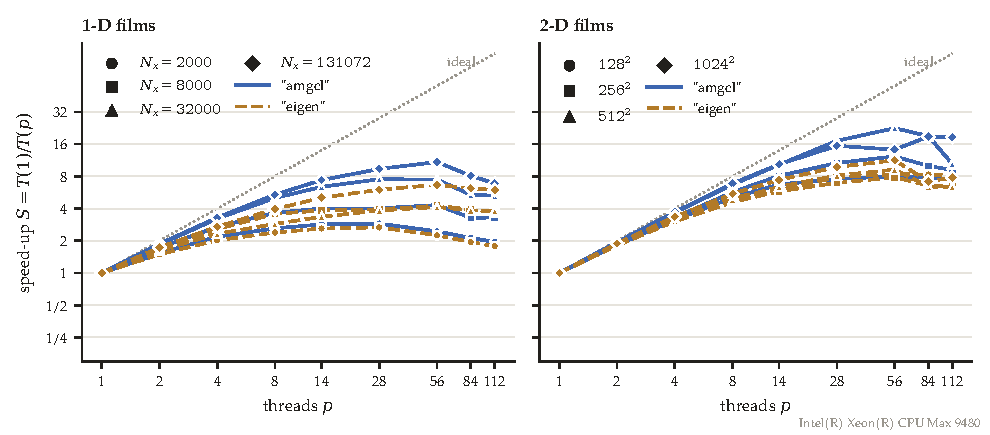
\includegraphics[width=\textwidth]{figures/parallel-scaling.pdf}
  \caption{\cref{tab:scaling}の速度向上率とスレッド数の関係（全規模、両バック
    エンド）。点線は理想値$S = p$である。大きな液膜では両バックエンドともスケールし、
    \val{"amgcl"}のほうがよく伸びる。小さな1次元の液膜は$3\times$付近で頭打ちになる。
    1ソケット（56スレッド）を超えると、ほとんどのケースで低下する。
    \file{tools/scaling/\bk results/\bk scaling-mc076.tsv}をもとに
    \file{docs/manual/\bk figures/\bk make\_scaling.py}で作図した。\label{fig:parallel-scaling}}
\end{figure}

同じ数値を曲線にしたものが\Cref{fig:parallel-scaling}である。ここから次の四点が読み取れる。

\paragraph{両バックエンドともスケールし、\val{"amgcl"}のほうがよく伸びる。}
2次元の56スレッドでは、\val{"eigen"}は$8\times$から$11\times$、\val{"amgcl"}は
$8\times$から$22\times$に達し、液膜が大きいほど倍率も大きい。\val{"eigen"}の前処理は
ブロックを並列に分解するブロック・ヤコビILUTである（\cref{sec:linsolve:eigen}）。
伸びを抑えているのはBiCGStab反復である。反復はループの33から\SI{72}{\percent}を占め、
そのベクトル演算は逐次に行う（\cref{sec:parallel:profile}）。AMGCLはセットアップも反復も
スレッド化している。

\paragraph{どちらのバックエンドが速いかはスレッド数による。}
1次元の$N_x = 2000$では、AMGCLが系を直接解くため両者は互角である（一スレッドで
\SI{9}{\percent}以内、28スレッドで\SI{2}{\percent}以内）。$8000$から$32000$では、
どのスレッド数でも\val{"eigen"}が速い。$N_x = 8000$での差は一スレッドで$5.8\times$、
56スレッドで$5.7\times$である。1次元の問題ではAMGCLが粗視化できる余地がほとんどなく、
求解一回に約100回の線形反復を要する。Eigenは12回で済む。
$N_x = 131072$では、一スレッドでの差は\SI{11}{\percent}以内であり、56スレッドでは
\val{"amgcl"}が$1.5\times$速い。2次元では、$128^2$で両者は互角である。$256^2$以上では、
一スレッドなら\val{"eigen"}が速く（$256^2$で$1.4\times$、$512^2$で$1.6\times$、
$1024^2$で$1.2\times$）、八スレッドでも$512^2$までは\val{"eigen"}が速い。8から28
スレッド以上になると\val{"amgcl"}が速い（$256^2$の56スレッドで$1.1\times$、$512^2$で
$1.5\times$、$1024^2$の28スレッドで$1.4\times$）。これを規則の形にまとめたものを
\Cref{sec:parallel:backend}に示す。

\paragraph{効果のあるスレッド数は112ではなく28--56である。}
一つを除くすべてのケースは、56スレッドまでに最適値に達するか、それを過ぎている。112
スレッドでは56スレッドより遅い。2ソケットには8個のNUMAノードがあり、1ソケットを
超えると、縮約とメモリトラフィックのコストがコアを増やした効果を上回る。一回の計算で
使うのを1ソケットまでとしているのはこのためである（\cref{sec:parallel:cap}）。例外は
$1024^2$の\val{"amgcl"}で、84スレッドで最速となり、28スレッドより時間が\SI{18}{\percent}
短い。56スレッドでは3回の繰り返しに\SI{22}{\percent}のばらつきがあった。（$N_x = 2000$の
\val{"amgcl"}の行は、AMGCLの最も粗いレベルを修正したあと、同種の別のノードで測り直した。
そのノードで計時した\val{"eigen"}は、\cref{tab:scaling}と\SI{2}{\percent}以内で一致した。）

\paragraph{小さな問題は並列化の効果がない。}
$N_x = 2000$での最良の速度向上率は、\val{"eigen"}で$2.7\times$、\val{"amgcl"}で
$2.9\times$であり、いずれも28スレッドのときである。それ以上スレッドを増やすと、かえって時間がかかる。
格子点が数千未満なら、ケースごとに一スレッドで実行し、複数のケースを並行して流すべきである。
なお、\cref{tab:scaling}の測定ではスレッド上限を無効にしているので、どの行も指定した
スレッド数で実行した結果である。

\begin{note}[集計ツールのアムダール近似の読み方]
  \file{tools/scaling/summarize.py}は、当てはめで得た並列化率$f$を出力する。最適値を
  過ぎて遅くなるケースでは$f = 0.000$と報告されるが、これは何も並列化されて
  いないという意味ではない。アムダールの法則は飽和を表せても減速は表せないため、
  回帰で当てはめる対象がないのである。モデルにすぎない$f$より、実測値である$S$と$E$を
  参照されたい。
\end{note}

\section{バックエンドの選び方}
\label{sec:parallel:backend}

上の測定から次の規則が得られる。選択を誤ったときの損失が大きいのは1次元だけである。
2次元では、1ソケット分までのスレッド数とすべての規模で、両バックエンドの差は1.6倍以内に
収まる。

\begin{yzntable}{問題の形状によるバックエンドの選択\label{tab:backend-rule}}{@{}L{0.22\textwidth} L{0.16\textwidth} L{0.50\textwidth}@{}}
\textsf{\bfseries 問題} & \textsf{\bfseries バックエンド} & \textsf{\bfseries 理由}\\ \midrule
1次元、$\sim 10^4$--$10^5$セルまで & \val{"eigen"} & AMGCLでは粗視化の余地がほとんどなく、線形反復が8倍に増える。$N_x=8000$で$5.7\times$遅い。AMGCLが直接解く$N_x = 2000$では互角。 \\
1次元、$\sim 10^5$セル以上 & どちらでも & 一スレッドで\SI{11}{\percent}以内。$N_x = 131072$の56スレッドでは\val{"amgcl"}が$1.5\times$速い。 \\
2次元、1ソケット分のスレッド & \val{"amgcl"} & $256^2$以上で$1.1$--$1.5\times$速く、$128^2$では互角。 \\
2次元、八スレッド以下 & \val{"eigen"} & $256^2$以上では一スレッドで$1.2$--$1.6\times$速い。 \\
\end{yzntable}

\val{"auto"}は液膜の面内の次元を見て、1次元なら\val{"eigen"}、2次元なら
\val{"amgcl"}を選ぶ。既定値は\val{"auto"}なので、キーを設定しなければ、1次元では
$\sim 10^5$セル未満のとき、2次元では1ソケットをすべて使うときに、速いほうのバックエンドに
なる。小さな計算機で$256^2$以上の2次元の液膜を計算する場合は、\key{Backend}を
\val{"eigen"}に設定する必要がある。

\begin{note}[規模やスレッド数のしきい値がない理由]
  一方のバックエンドが他方を追い越す点は計算機によって異なり、1次元以外ではどちらを
  選んでも得られる差は小さい。しきい値を設けると、計算機に依存する推測をソルバーに持ち込む
  ことになる。そのため\val{"auto"}は次元だけで判断する。長期にわたる研究で計算時間が重要なら、
  自分の計算機で両方を測定し（\cref{sec:parallel:kit}）、\key{Backend}を明示的に設定されたい。
\end{note}

\section{自分の計算機での測定}
\label{sec:parallel:kit}

この測定のために、自己完結したキット\file{tools/scaling/}を用意している。ケースの生成、
掃引スクリプト、集計ツールからなる。

\begin{shell}
cmake -S . -B build -DCMAKE_BUILD_TYPE=Release -DYUZEN_WITH_AMGCL=ON
cmake --build build -j

tools/scaling/scaling.sh --tier quick --repeats 1 --threads "1 4"
tools/scaling/scaling.sh --threads "1 2 4 8 16 32 64" --repeats 3
python3 tools/scaling/summarize.py tools/scaling/results/scaling-*.tsv
\end{shell}

掃引スクリプトは、計算一回ごとに1行をタブ区切りファイルに追記する。ファイルのヘッダーには
計算機の識別情報を記録し、既にある行は飛ばす。そのため、中断した掃引は同じコマンドを
もう一度実行すれば再開できる。各ケースは仕事量を固定しており、そのおかげで数値を
比較できる。時間刻みは一定（\key{Numerics.TimeStepControl}は無効）、ステップ数は固定
（\key{Numerics.MaxSteps}）とし、場の出力は無効にしてある。出力間隔は時間刻みの上限にも
なるので、出力を有効にすると、書き込みの時間だけでなくステップあたりの仕事量も変わってしまう。
計時の対象はプロセス全体ではなく、\file{JobInfo.txt}に記録された時間刻みループの時間だけである。
したがって、格子の構築や起動処理の時間が結果に混ざることはない。

\begin{warn}[小さなケースでは、どうしても大きな計算機を使いきれない]
  \code{Vector}の縮約では、答えがスレッド数に依存しないよう、$N$要素を
  $\min(256,\,N/512)$個の固定数のブロックに分割する（\cref{sec:repro:reduction}）。
  ここから二つの制約が生じる。まず、未知数が$512p$未満のケースでは、$p$スレッドすべてに
  ブロックを割り当てることができない。112スレッドでは57\,344未知数が必要であり、
  ブロック数が上限に達するだけの余裕をもたせるには131\,072が要る。また、上限が256ブロック
  なので、\textbf{256スレッドを超えると縮約はそれ以上並列化しない}。この上限は
  ビット単位の一致と引き換えであり、意図して設けている。

  キットの規模を2次元で$1024^{2}$、1次元で$N_x =
  131\,072$まで用意しているのはこのためである。小さなケースは逆の側を示すために含めている。
  つまり、小さなケースは並列化しても速くならず、一スレッドずつ複数を同時に実行すべきだということである。
\end{warn}

\subsection{時間の内訳}
\label{sec:parallel:profile}

\env{YUZEN\_PROFILE=1}とすると、ソルバーは処理の各部分を名前付きで計時し、終了時に合計を
標準エラーへ1行ずつ（名前、呼び出し回数、秒数）書き出す。
\begin{shell}
[profile] threads 8
[profile] h.linsolve        2030      0.097730
\end{shell}
\begin{yzntable}{\env{YUZEN\_PROFILE}が計時する部分。入れ子になった部分の時間は内側の部分を含む。たとえば\code{h.linsolve}は膜厚の\code{lin.*}を含む。\label{tab:profile-parts}}{@{}L{0.20\textwidth} L{0.72\textwidth}@{}}
\textsf{\bfseries 名前} & \textsf{\bfseries 内容}\\ \midrule
\code{step}        & 1時間刻みの全体 \\
\code{output}      & ステップ間の場と履歴の出力 \\
\code{h.assemble}  & 膜厚の行列（\code{SetMatrixA}） \\
\code{h.jacobian}  & 膜厚の行列のヤコビアンと、陰的ステップの行列 \\
\code{h.rhs}       & 陽的部分と右辺 \\
\code{h.linsolve}  & 膜厚の線形求解 \\
\code{h.couple}    & ニュートンパスの残り（鉛直一様モデルの濃度の試行計算を含む） \\
\code{h.after}     & ステップ終了時の処理（そのステップの濃度計算を含む） \\
\code{c.solve}     & 濃度の求解の全体。うち線形求解が\code{c.linsolve} \\
\code{velocity}    & 速度 \\
\code{lin.prepare} & バックエンドへの行列の受け渡し（収集、スケーリング、コピー） \\
\code{lin.precond} & 前処理の構築（ILUT分解、AMGのセットアップ） \\
\code{lin.iterate} & BiCGStab反復 \\
\end{yzntable}
並列領域の内側に置いた計時スコープは何も測らない。計時の対象は、時間ループを実行している
スレッドから見える範囲である。\file{tools/profile\_threads.py}は、\cref{sec:parallel:cap}の
上限を無効にしたうえで、一組のケースを両バックエンド、各スレッド数で実行し、各部分の時間を
スレッド数ごとに表にまとめる。バッチの時間制限に収まるよう、\file{tools/case\_runtimes.py}と
同じく分割して測定する（\cref{sec:env:tools}）。

\cref{tab:scaling}と同様のXeon Max 9480ノードでこのツールを使うと、
\cref{sec:parallel:scaling}で見た限界の原因が明らかになる。\cref{tab:scaling}の2次元の
液膜で\val{"eigen"}を使う場合、ブロック・ヤコビILUT前処理の構築が時間刻みループの
6--30\,\%（小さな格子ほど大きい）、BiCGStab反復が33--72\,\%
（大きな格子ほど大きい）を占める。\file{leveling\_2d\_reg}の$60\times60$の液膜では、
分解が55--61\,\%を占める。四スレッド以上ではブロックが仕事を分割しなくなるためである。
\val{"amgcl"}では、AMGのセットアップを線形求解のたびに、つまり1ステップに五回から
八回（膜厚で約三回、濃度で二回から四回）作り直す。セットアップは反復よりもスケールしにくく、
ループに占める割合は一スレッドの4--9\,\%から56スレッドの10--28\,\%に増える。
割合は小さな格子ほど大きい。バックエンドへの行列の受け渡しは、2次元のケースでは
どのスレッド数でも0--3\,\%である。

\section{速度と再現性は別の問題である}
\label{sec:parallel:repro}

スレッド数を変えても答えは変わらない。\val{"eigen"}では結果がビット単位で一致し、
テストスイートで確認している（\cref{ch:reproducibility}）。\val{"amgcl"}では
末尾の数桁が動く（\cref{sec:verification:amgclthreads}）。つまり、スレッド数は
性能だけを考えて選べば十分である。正しさにかかわるのはバックエンドの選択のほうである。
スレッド数だけでなく計算機が変わってもビット単位で一致する結果が必要なら、
バックエンドを\val{"eigen"}に固定し、2次元の求解が遅くなることは受け入れる必要がある。
